\chapter*{Appendix}

\begin{figure}
	\centering
		
\includegraphics[width=0.7\textwidth]{gt_surgeon_example.png}
	\caption{Google Translate assigns stereotypical genders to occupational roles.}
	\label{fig:gt_surgeon_example}
\end{figure}

\begin{figure}
	\centering
		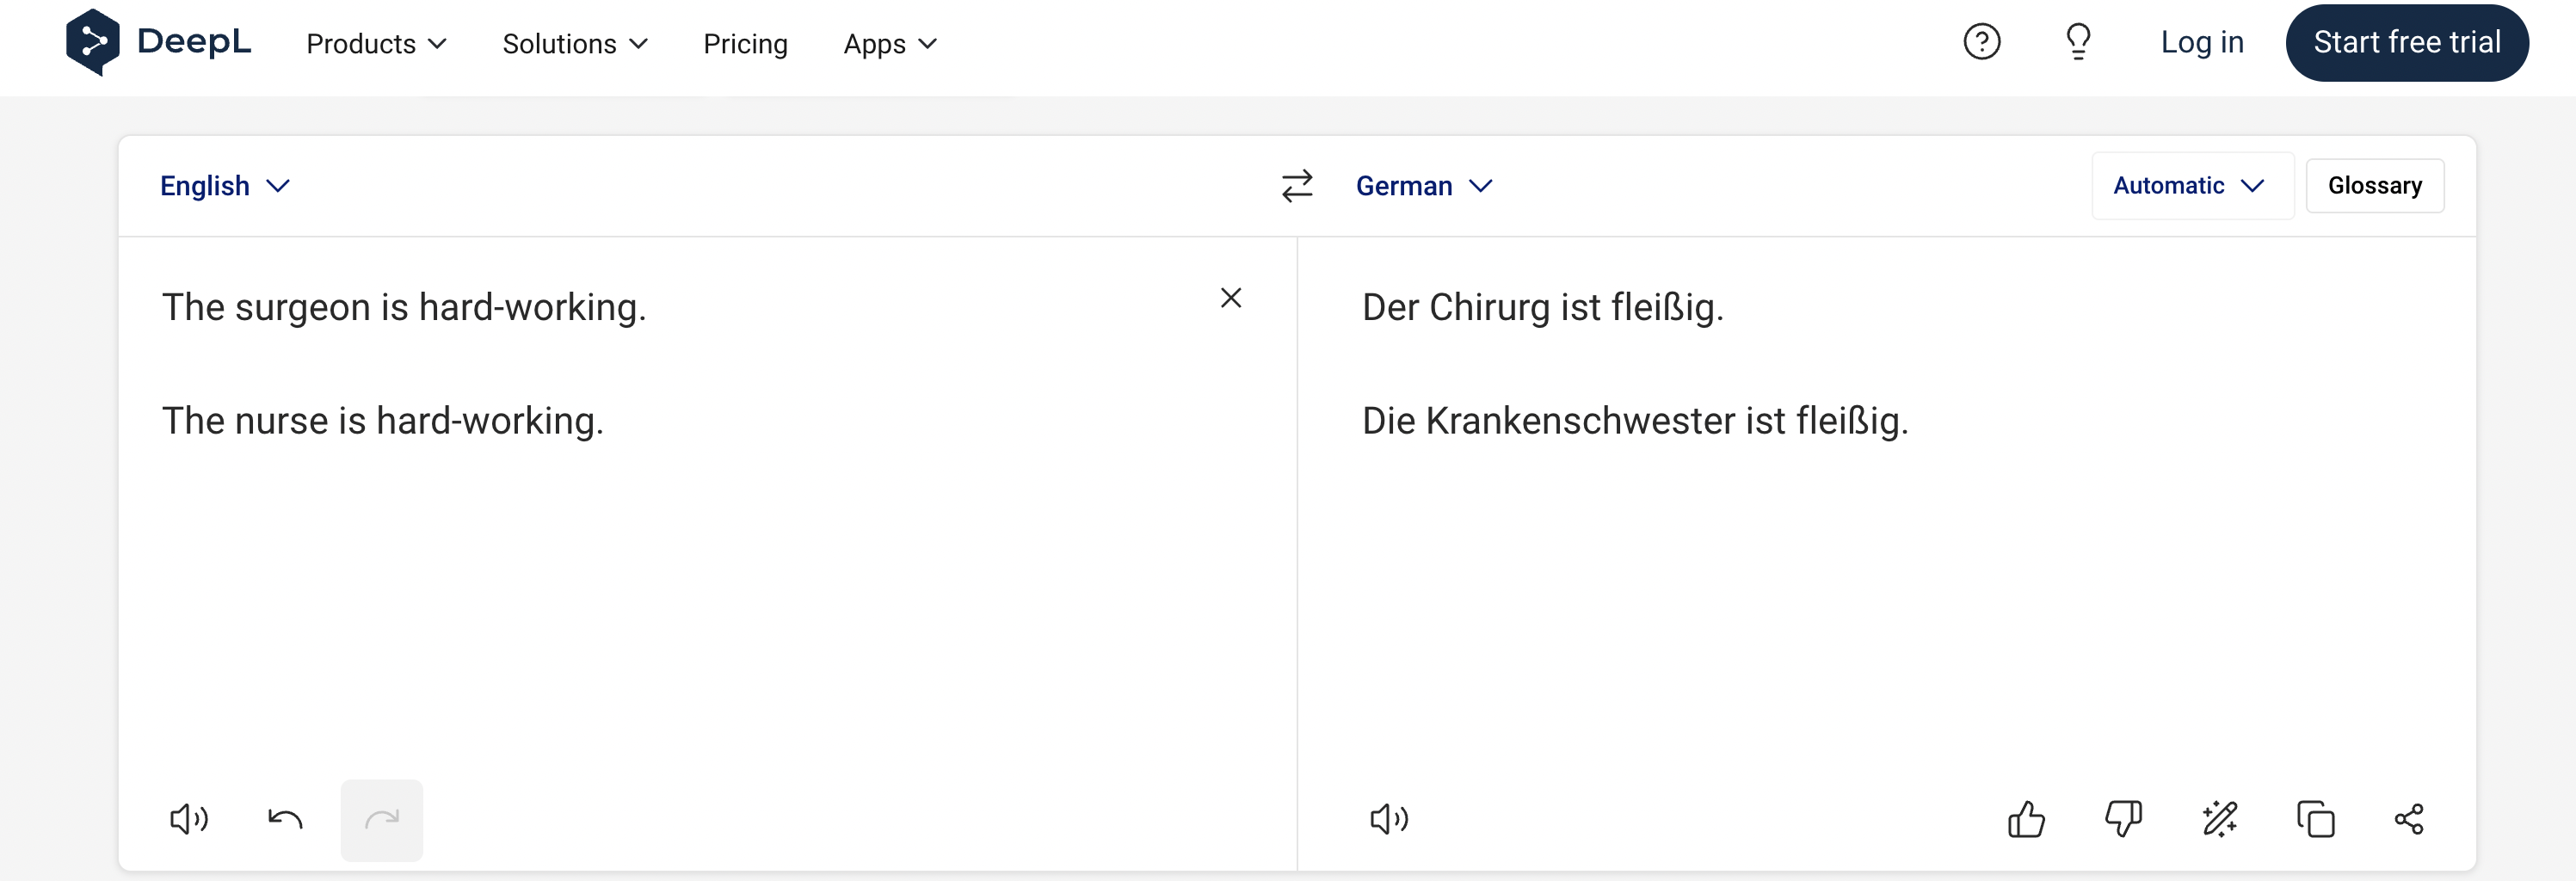
\includegraphics[width=0.7\textwidth]{deepL_surgeon_example.png}
	\caption{DeepL shows a similar bias in the same sentence, highlighting consistent patterns across MT tools.}
	\label{fig:deepL_surgeon_example}
\end{figure}

\begin{figure}
	\centering
		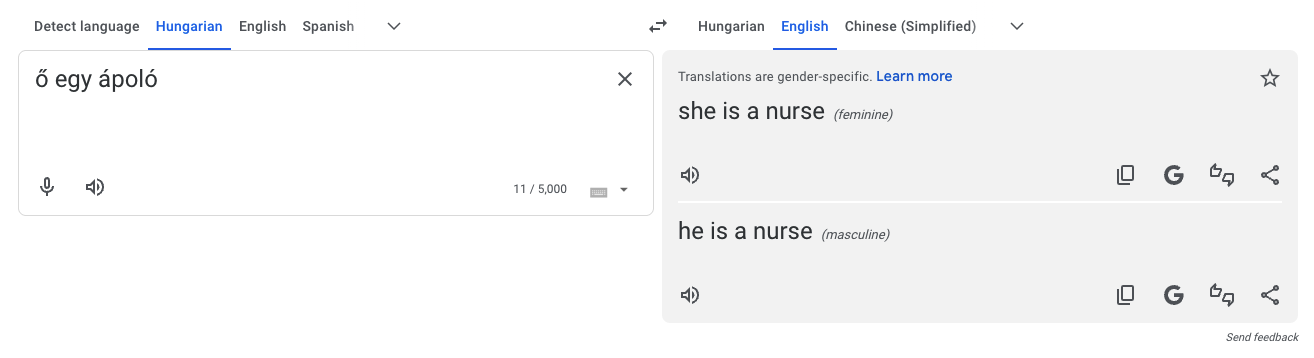
\includegraphics[width=0.7\textwidth]{gt_prates_example.png}
	\caption{Gender-specific translation by Google Translate for ambiguous pronouns.}
	\label{fig:gt_prates_example}
\end{figure}

\section{Prompt and Output for Pre-training/Fine-tuning Explanation}
\label{appendix:prompt_pdf}
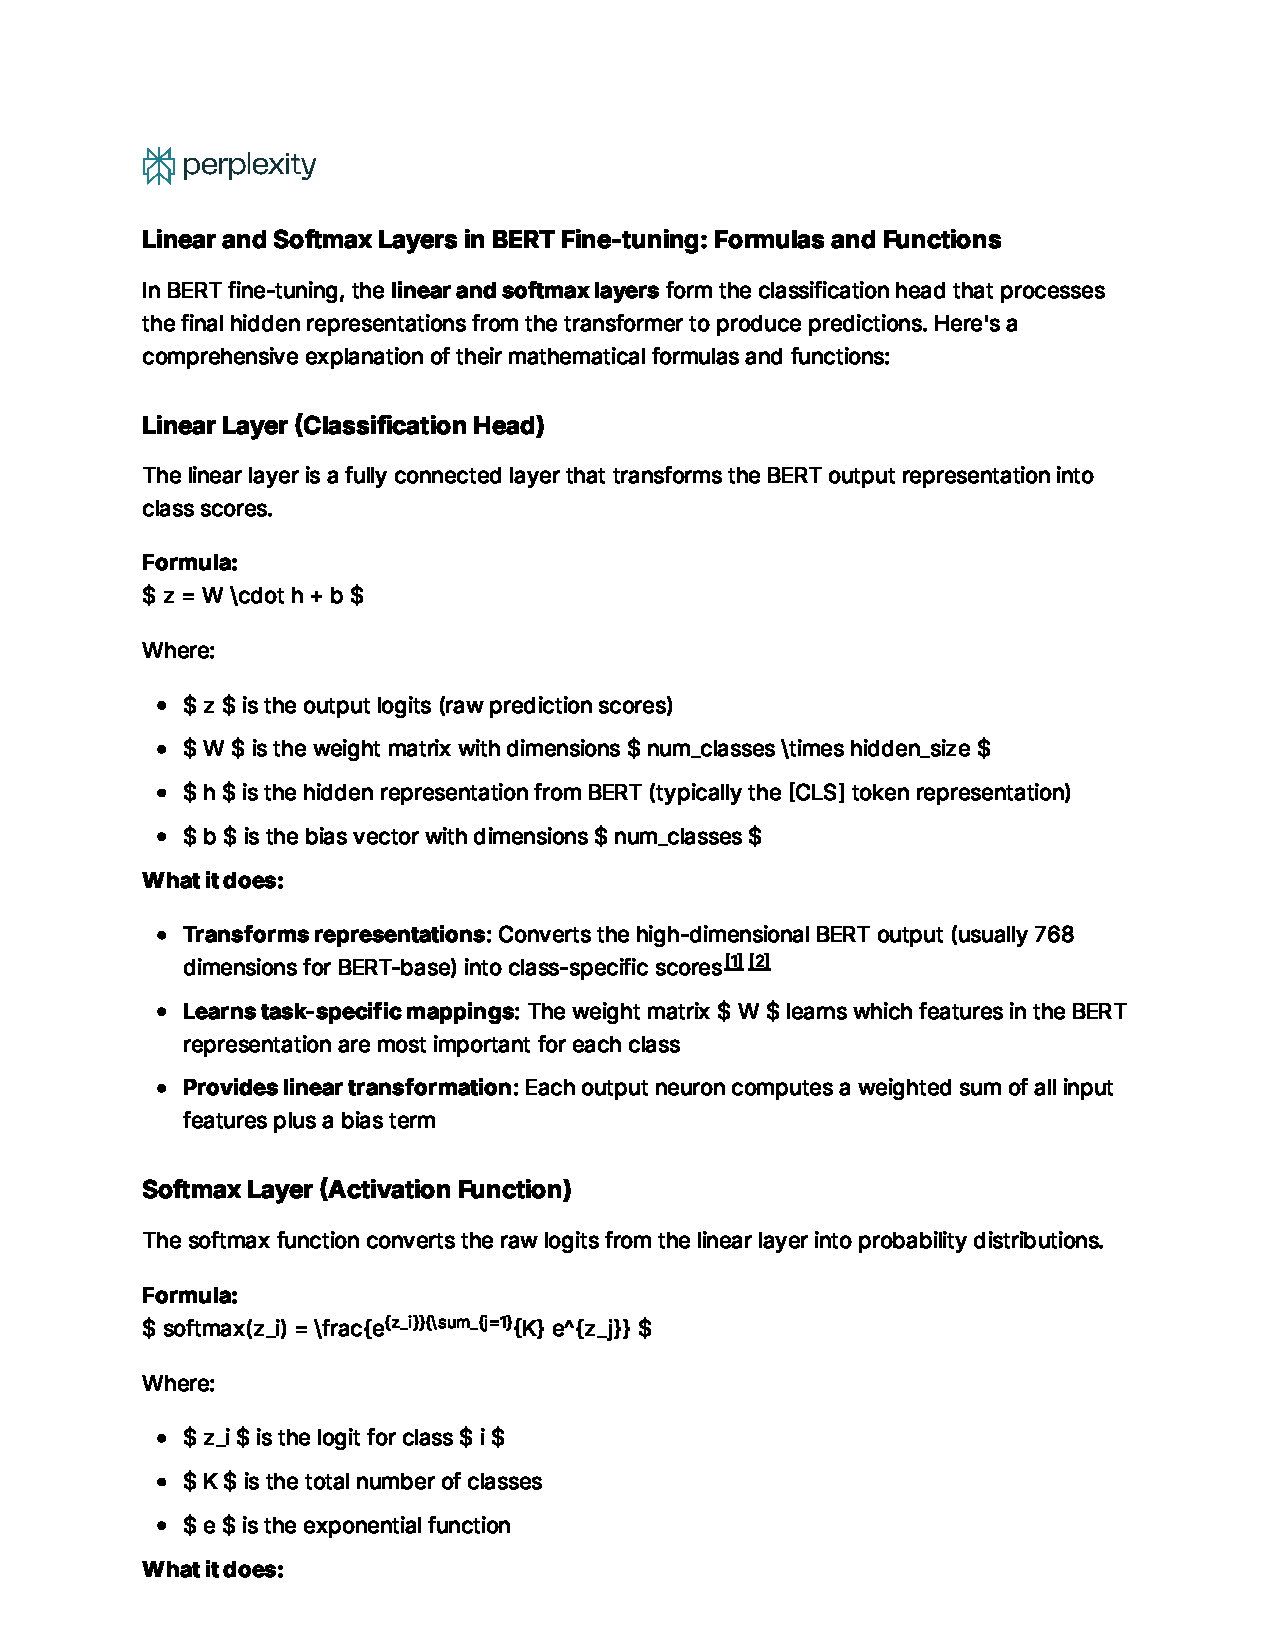
\includepdf[pages=-]{./Literatur/Linear and Softmax 14-jul-2025.pdf}